\documentclass[tikz,border=6pt]{standalone}
\usepackage[utf8]{inputenc}
\usepackage{amsmath}
\usetikzlibrary{positioning,arrows.meta,calc}
\begin{document}
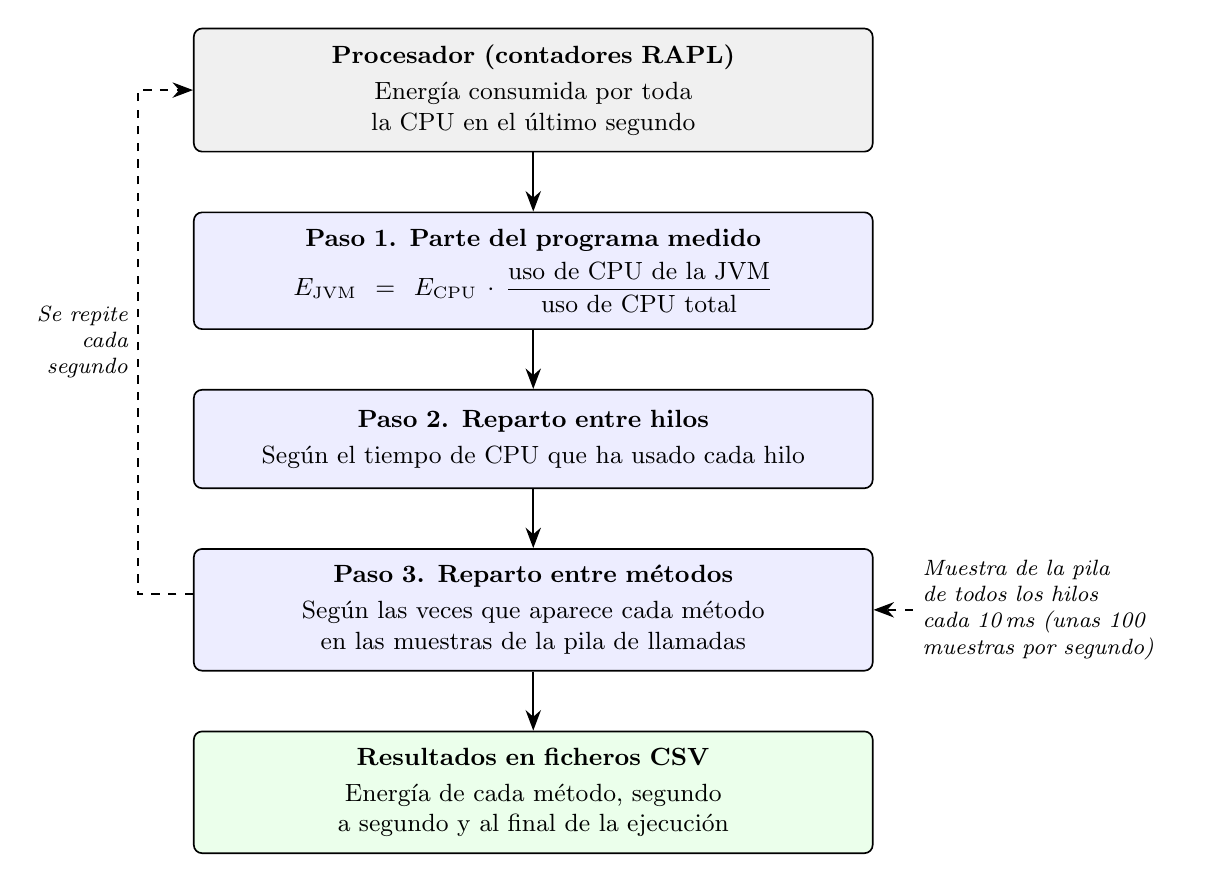
\begin{tikzpicture}[
  font=\small,
  box/.style={draw, rounded corners=3pt, align=center, text width=8.2cm,
              minimum height=1.25cm, inner sep=6pt, line width=0.6pt},
  src/.style={box, fill=gray!12},
  paso/.style={box, fill=blue!7},
  salida/.style={box, fill=green!8},
  arr/.style={-{Stealth[length=2.6mm]}, line width=0.7pt},
  lbl/.style={font=\footnotesize\itshape, align=left, text width=3.4cm}
]
\node[src]  (cpu) {\textbf{Procesador (contadores RAPL)}\\[2pt]
  Energía consumida por toda la CPU en el último segundo};
\node[paso, below=0.75cm of cpu] (p1) {\textbf{Paso 1. Parte del programa medido}\\[3pt]
  $E_{\text{JVM}} = E_{\text{CPU}} \cdot
   \dfrac{\text{uso de CPU de la JVM}}{\text{uso de CPU total}}$};
\node[paso, below=0.75cm of p1] (p2) {\textbf{Paso 2. Reparto entre hilos}\\[2pt]
  Según el tiempo de CPU que ha usado cada hilo};
\node[paso, below=0.75cm of p2] (p3) {\textbf{Paso 3. Reparto entre métodos}\\[2pt]
  Según las veces que aparece cada método en las muestras de la pila de llamadas};
\node[salida, below=0.75cm of p3] (csv) {\textbf{Resultados en ficheros CSV}\\[2pt]
  Energía de cada método, segundo a segundo y al final de la ejecución};

\draw[arr] (cpu) -- (p1);
\draw[arr] (p1) -- (p2);
\draw[arr] (p2) -- (p3);
\draw[arr] (p3) -- (csv);

\node[lbl, right=0.5cm of p3] (samp) {Muestra de la pila\\de todos los hilos\\cada 10\,ms (unas 100\\muestras por segundo)};
\draw[arr, dashed] (samp.west) -- (p3.east);

\draw[arr, dashed] ($(p3.west)+(0,0.2)$) -- ++(-0.7,0) |- node[pos=0.25, left, font=\footnotesize\itshape, align=right]{Se repite\\cada\\segundo} ($(cpu.west)+(0,0)$);
\end{tikzpicture}
\end{document}
